% LaTeX-Vorlage Version 3.0,  Juni 2010
% erstellt von Dr. Andreas Drauschke und Dr. Susanne Teschl
% Modifiziert von Dr. Andreas Mehrle (andreas.mehrle@mci.edu)

%MODIFIZIERT von M. Panny - Version 1.8.0

\documentclass[a4paper, oneside, 10pt]{article}

\newcounter{RoemischeSeiten}
\pagenumbering{Roman}

\usepackage[dvips]{graphicx}
\usepackage[tmargin=1in,bmargin=1in,lmargin=1.25in,rmargin=1.25in]{geometry}
\usepackage{titlesec}
\usepackage{xcolor}
\usepackage[overload]{textcase}
\usepackage[utf8]{inputenc}
\usepackage{epstopdf}
\usepackage{listings}
\usepackage{wallpaper}
\usepackage[binary-units=true]{siunitx} %Zusätzliche Option erlaubt binary-units wie z.B.: \byte
\usepackage{placeins} %Für \FloatBarrier beim Einfügen von Abbildungen
%=============================================
\usepackage{exscale,relsize}
\usepackage{fancyhdr}
\usepackage[small]{caption}
\usepackage{float}
\usepackage{amsmath, amssymb, amsfonts, amsthm}
\usepackage{pst-all}
\usepackage{rotating}
\usepackage{mathrsfs}
\usepackage{makeidx}
\usepackage{multirow}
%=============================================
\usepackage{pgfplots}
\usepackage{tikz}
%\usepackage[european, siunitx]{circuitikz}
%=============================================
\usepackage{setspace} 
\usepackage{booktabs}
\usepackage{graphicx}
\usepackage{cancel}
\usepackage{xspace}
%=============================================
\usepackage{subcaption}
\usepackage{pdfpages}
\usepackage{nameref}
\usepackage[pdftex,bookmarks=true,bookmarksnumbered=true]{hyperref}
\usepackage{wasysym}
%=============================================
%STEINMETZ
%\PassOptionsToPackage{original}{pict2e} falls Probleme zw. cancel und steinmetz auftreten
\usepackage{steinmetz}	%für Versor/Phasor Symbol für Winkel in der Elektrotechnik 
%=============================================

%FONTS für \ttfamily und \bfseries gleichzeitig --> wird normal nicht unterstützt
%http://www.macfreek.nl/memory/LaTeX_Bold_Typewriter_Font
\DeclareFontShape{OT1}{cmtt}{bx}{n}{<5><6><7><8><9><10><10.95><12><14.4><17.28><20.74><24.88>cmttb10}{}

%SPRACHEN einrichten --> für Englisch: [main=english, ngerman] --> es muss evtl. 2x kompiliert werden
\usepackage[english]{babel}

\def\headerLists{headerLists}
\iflanguage{ngerman}{\def\headerLists{Verzeichnisse}}{}
\iflanguage{ngerman}{\def\headerLists{Indices}}{}
\iflanguage{ngerman}{\renewcommand\lstlistlistingname{Quellcodeverzeichnis}}{}
\iflanguage{ngerman}{\renewcommand\lstlistlistingname{List of \lstlistingname s}}{}
\expandafter\addto\csname captionsngerman\endcsname{\renewcommand{\refname}{Literaturverzeichnis}}

%Einstellung für TOC, damit lange Seitennummer (römisch) nicht zu weit rechts steht --> Wert muss angepasst werden
\makeatletter
\renewcommand{\@pnumwidth}{1.55em}	%default = 1.55em
\makeatother

%===================================================================

%FARBEN für Deckblatt, etc.
\def\isBlackAndWhite{1}
\if\isBlackAndWhite1
	\definecolor{MSBlue}{rgb}{0, 0, 0}
	\definecolor{MSLightBlue}{rgb}{0, 0, 0}
	%für listings
	\definecolor{lstGreen}{RGB}{0, 0, 0}
	\definecolor{lstBlue}{RGB}{0, 0, 0}
	\definecolor{lstGreenMatlab}{RGB}{0, 0, 0}
	\definecolor{lstLila}{RGB}{0, 0, 0}
\else
	\definecolor{MSBlue}{rgb}{0.204, 0.353, 0.541}
	\definecolor{MSLightBlue}{rgb}{0.31, 0.506, 0.741}
	%für listings
	\definecolor{lstGreen}{RGB}{46, 109, 103}
	\definecolor{lstBlue}{RGB}{40, 38, 160}
	\definecolor{lstGreenMatlab}{RGB}{28,172,0}
	\definecolor{lstLila}{RGB}{170,55,241}
\fi

%===================================================================

%FORMATS for each heading level
%\titleformat*{\section}{\rmfamily\bfseries\huge\color{MSBlue}\lowercase}
\setcounter{secnumdepth}{4}
\titleformat{\section}[hang]{\sffamily\bfseries\huge\color{MSBlue}}{\thesection}{1em}{}[]
\titleformat{\subsection}{\large\bfseries\sffamily\uppercase}{\thesubsection}{1em}{}
\titleformat{\subsubsection}{\sffamily\bfseries}{\thesubsubsection}{1em}{}
\titleformat{\paragraph}{\sffamily\bfseries}{\theparagraph}{1em}{}
\newcommand{\subsubsubsection}{\paragraph}
\titleformat{\subparagraph}{\sffamily\bfseries}{\thesubparagraph}{1em}{}
\newcommand{\subsubsubsubsection}{\subparagraph}

%\newcommand{\subsubsubsection}{\textbf}
%===================================================================

%SIUNITX
\iflanguage{ngerman}{\sisetup{locale=DE, tophrase={~bis~}}}{}		%Macht z.B.: Komma zum Dezimalseparator
\DeclareSIUnit{\var}{var}	%Volt-Ampere-Reaktiv
\DeclareSIUnit{\VA}{VA}		%Volt-Ampere
\DeclareSIUnit{\Nm}{\newton \meter}		%Newtonmeter
\DeclareSIUnit{\mm}{\milli \meter}		%Millimeter
\DeclareSIUnit{\Npsmm}{\newton \per \square \milli \meter}	%Newton-pro-Quadratmillimeter
\DeclareSIUnit{\decade}{dec}
%===================================================================

%LISTINGS for inline source code highlighting
\lstdefinelanguage{ST}{	%settings für Strukturierten Text
	keywords = {
		PROGRAM, CONFIGURATION, END_CONFIGURATION, VAR, VAR_GLOBAL, VAR_EXTERNAL, END_VAR, TASK, INTERVAL, AT, EXIT, WITH, VAR_INPUT, VAR_OUTPUT,
		IF, ELSE, ELSIF, THEN, END_IF, CASE, OF, END_CASE, RETURN,
		REPEAT, UNTIL, END_REPEAT, WHILE, END_WHILE, FOR, END_FOR, DO, TO, BY,
		BOOL, BYTE, WORD, DWORD, LWORD,
		INT, SINT, DINT, LINT, USINT, UINT, LDINT, ULINT, 
		REAL, LREAL, 
		ADR, TRUNC, ABS, SQRT, LN, LOG, EXP, SIN, COS, TAN, ASIN, ACOS, ATAN, EXPT,
		STRING, TIME, DATE, TIME_OF_DAY, DATE_AND_TIME,
		NOT, AND, OR, XOR, TRUE, FALSE, MOD, EXPT, FUNCTION_BLOCK
	},
	sensitive = true,			%case sensitivity --> should probably be false
	morecomment = [l]{//},		%inline comment
	morecomment = [s]{(*}{*)},	%mult line comment
	morecomment = [s]{/*}{*/},
	morestring = [b]",
	morestring = [b]',
	tabsize = 4
}

%default style for ST --> language must not be specified when using style
\lstdefinestyle{ST}{
	language=ST,
	basicstyle=\small\ttfamily,
	keywordstyle=\color{lstBlue}\bfseries,
	columns=fullflexible,
	breaklines=true,
	postbreak=\mbox{$\hookrightarrow$\space},
	captionpos=t,	%t for top or b for bottom
	commentstyle=\color{lstGreen}\itshape,
}

%default style for MATLAB --> language must not be specified when using style
\lstdefinestyle{matlab}{
	language=Matlab,
	basicstyle=\small\ttfamily,
	keywordstyle=[1]\color{lstBlue}\bfseries,
	keywordstyle=[2]\color{lstLila},
	commentstyle=\color{lstGreenMatlab}\itshape,
	stringstyle=\color{lstLila},
	showstringspaces=false,
	captionpos=t,
	tabsize = 4,
	columns=fullflexible,
	breaklines=true,
	postbreak=\mbox{$\hookrightarrow$\space},
	morekeywords={xlim,ylim,var,alpha,factorial,poissrnd,normpdf,normcdf,clearvars},
	%Put MATLAB function parameters here
	morekeywords=[2]{step_PT1, step_PT1T, step_PT2},
	morecomment=[l][\color{blue}]{...},     % Line continuation (...) like blue comment
}

%===================================================================

%TIKZ
\newcommand{\tikzDrawBB}{\draw (current bounding box.north east) -- (current bounding box.north west) -- (current bounding box.south west) -- (current bounding box.south east) -- cycle;}

%===================================================================
\numberwithin{figure}{section}
\numberwithin{table}{section}

% auxillary symbols
\renewcommand{\tilde}{\symbol{126}}
\newcommand{\define}{\stackrel{!}{=}}
\renewcommand{\equiv}{\,\widehat{=}\,}

\newcommand{\im}{j}
\newcommand{\matlab}{MATLAB\xspace}
\newcommand{\labview}{LabVIEW\xspace}
\newcommand{\simulink}{Simulink\xspace}
\newcommand{\flexsim}{FlexSim\xspace}

% format specifications
\newcommand{\ten}[1]{\mathbf{#1}}	%Tensor
\newcommand{\mat}[1]{\mathbf{#1}}	%Matrix

% mathematical operators
\newcommand{\grad}{\,\mathrm{grad}\,}
\renewcommand{\div}{\,\mathrm{div}\,}
\newcommand{\rot}{\,\mathrm{rot}\,}
\newcommand{\lap}{\Delta}
\newcommand{\laplace}[1]{\mathscr{L}\left\{#1\right\}}	%Laplacetransformation
\newcommand{\invLaplace}[1]{\mathscr{L}^{-1}\left\{#1\right\}}	%inverse Laplactransformation
\newcommand{\trans}{^{\raisebox{\depth - 0.075em}{$\intercal$}}}%{^T}	%Transponiert --> für Matrix
\DeclareMathSymbol{*}{\mathbin}{symbols}{"01} % Punkt statt *

%===================================================================

%Grad als Einheit --> °
\newcommand{\gradU}[1]{\SI{#1}{\degree}} %hauptsächlich in kombination mit steinmetz-package sinnvoll

%Toleranzen
\newcommand{\tol}[4]{\ensuremath{\SI{#1}{#2}^{+\num{#3}}_{-\num{#4}}}}	%#1 #2 +#3 -#4
\newcommand{\tolSingle}[3]{\ensuremath{\SI{#1}{#2}^{+\num{#3}}}}

%command für römische Zahlen
\newcommand{\RN}[1]{\textup{\uppercase\expandafter{\romannumeral#1}}}

%circled numbers (normal, big and small)
\newcommand{\circText}[1]{{\large \textcircled{\small{#1}}}}
\newcommand{\circTextBig}[1]{{\Large \textcircled{\normalsize{#1}}}}
\newcommand{\circTextSmall}[1]{{\textcircled{\small{#1}}}}

%command für dx, etc. für Integral
\newcommand{\diff}{\mathop{}\!\mathrm{d}}	%\diff x --> dx
\newcommand{\Diff}[1]{\mathop{}\!\mathrm{d^{#1}}} %\Diff[2] x --> d²x

%command für Ableitungen (normal und partiell) --> Verwendung austauschbar:
%\deriv{I}{t} --> dI/dt
%\deriv[2]{s}{t} --> d^2 s/dt^2
\newcommand{\deriv}[3][]{\frac{\Diff{#1} #2}{\diff {#3}^{#1}}}
\newcommand{\parDeriv}[3][]{\frac{\partial^{#1} #2}{\partial {#3}^{#1}}}

%command für nicht kursives e im Mathmode --> soll nicht kursiv sein, da eine Konstante
\newcommand{\eUpr}{\mathrm{e}}

%===================================================================
%ENVIRONMENTS

%small matrix mit eckigen Klammern
\newenvironment{bsmallmatrix}{\left[\begin{smallmatrix}}{\end{smallmatrix}\right]}

%===================================================================

\setlength{\parindent}{0em}
\setlength{\parskip}{1.5ex plus0.5ex minus0.5ex}
\setlength{\captionmargin}{3em}

\newcommand{\textdirectcurrent}{%
	\settowidth{\dimen0}{$=$}%
	\vbox to .85ex {\offinterlineskip
		\hbox to \dimen0{\leaders\hrule\hfill}
		\vskip.35ex
		\hbox to \dimen0{%
			\leaders\hrule\hskip.2\dimen0\hfill
			\leaders\hrule\hskip.2\dimen0\hfill
			\leaders\hrule\hskip.2\dimen0
		}
		\vfill
	}%
}
\newcommand{\mathdirectcurrent}{\mathrel{\textdirectcurrent}}







%============================= MATLAB STYLE ======================================
\lstdefinestyle{MStyle}{
    backgroundcolor=\color{backgroundColour},   
    language=Matlab, 
%    frame=single,
    basicstyle=\small\ttfamily,
    keywordstyle=[1]\color{Blue}\bfseries,  % MATLAB functions
    keywordstyle=[2]\color{Purple},         % MATLAB function arguments
    keywordstyle=[3]\color{Blue}\underbar,  % User functions
    identifierstyle=,                       % Nothing special about identifiers
    commentstyle=\usefont{T1}{pcr}{m}{sl}\color{MyDarkGreen}\small,
    stringstyle=\color{Purple},
    %%% Put standard MATLAB functions not included in the default
   %%% language here
    morekeywords={xlim,ylim,var,alpha,factorial,poissrnd,normpdf,normcdf},
    %%% Put MATLAB function parameters here
    morekeywords=[2]{on, off, interp},
    %%% Put user defined functions here
    morekeywords=[3]{FindESS, homework_example},
    morecomment=[l][\color{Blue}]{...},     % Line continuation (...) like blue comment
    numbers=left,
    firstnumber=1,
    numberstyle=\tiny\color{mGray},
    numbersep=5pt,
    stepnumber=5,
    showspaces=false,                
    showstringspaces=false,
    showtabs=false,                  
    tabsize=2,
}

\usepackage{xcolor}
\definecolor{Purple}{rgb}{0.71,0,1}
\definecolor{Black}{rgb}{0,0,0}
\definecolor{Blue}{rgb}{0,0,1}
\definecolor{mGreen}{rgb}{0,0.6,0}
\definecolor{mGray}{rgb}{0.5,0.5,0.5}
\definecolor{mPurple}{rgb}{0.58,0,0.82}
\definecolor{backgroundColour}{rgb}{0.95,0.95,0.92}
\definecolor{MyDarkGreen}{rgb}{0,0.8,0}
%============================= MATLAB STYLE ======================================


% LABORTITEL
\def\thesis{Report}
\def\labtitle{Laboratory Advanced Control Engineering}
\def\labcode{BB MECH-M-1-RTV-RTV-LB}
\def\labdate{13.01.2024 and 02.02.2024}

% LABORNAME & NUMMER
\def\labname{Lab 1 - Aerodynamic Levitation}
%\def\labnum{2}

% ANGABEN ZUM Studium & Student
\def\study{Master Mechatronics \& Smart Technologies}
\def\term{1.}
\def\lecturer{Jasper Volmer}
\def\group{MA-MECH-23-BB-2B}
\def\student{Lukas Figl, Lukas Sieß, Stefan Widmann}

\begin{document}

%\layout
\setlength{\belowcaptionskip}{-8pt}
 %Abstand nach Abbildungen von 0.0pt auf -8pt verringern

% Kopf- und Fusszeilen initiieren
\pagestyle{plain}

\thispagestyle{empty}
\sffamily

\ThisTileWallPaper{\paperwidth}{\paperheight}{Images/MCIHintergrundKPL.pdf}
%\put(-30,-685){\includegraphics[width=1.15\linewidth]{BG}}

{
	\bfseries

	\vspace*{3.5cm}

	\textcolor{MSBlue}{\sffamily\bfseries\huge\thesis}%

	\vspace*{0.5cm}

	\begin{doublespace} 
		
\textbf{\labtitle{} (\labcode)}

\textbf{\labname}

\textbf{\labdate}	

%Labor \labnum

	%\maketitle
	\vspace*{10cm}

	\textcolor{gray}{\study}

	\def\termname{Semester}
	\textcolor{gray}{\term{ }\termname}

	\def\lecturername{Lector}
	\textcolor{gray}{\lecturername: \lecturer}

	\def\groupname{Group}
	\textcolor{gray}{\groupname: \group}

	\def\authorname{Authors}
	\textcolor{gray}{\authorname: \student}

	\textcolor{gray}{\today}
	\end{doublespace} 
	\newpage
}

\newpage
\tableofcontents
\newpage

% Kopf- und Fusszeilen initiieren
% Inhalt einbinden

\pagestyle{fancy}
\setcounter{RoemischeSeiten}{\value{page}}
\pagenumbering{arabic}


% A short description of the experimental set-up with an image
\section{Introduction} \label{sec:introduction}
% A short description of the experimental set-up with an image
The corresponding laboratory \textit{Aerodynamic Levitation} to the course \textit{Advanced Control Engineering 1} gives students the opportunity to model a physical system using system identification method, create the according state space model, implement a state observer, design a state-feedback controller and implement and simulate everything with MATLAB and Simulink Coder. \cite{Laborleitfaden}

The aerodynamic levitation system (figure \ref{fig:setupLevitation}) consists of a table tennis ball, a transparent hollow cylinder with a blower fan and an infrared distance sensor on the top. By controlling the speed of the blower fan, the height of the table tennis ball can be specified. Additionally, a National Instruments data acquisition card as well as a fan speed control system in combination with laboratory power supplies are used for this laboratory. \cite{Laborleitfaden}

\FloatBarrier
\begin{figure}[ht]
	\begin{center}
		\includegraphics[width=0.7\textwidth]{figure/setupLevitation.jpg}
		\caption[Aerodynamik levitation system setup \cite{Laborleitfaden}]
                {Aerodynamik levitation system setup \cite{Laborleitfaden}}
		\label{fig:setupLevitation}
	\end{center}
\end{figure}
\FloatBarrier

The lab preparation for the first session is to fit the sensor output based on the data given on Sakai (see figure \ref{fig:fittedFunction} in the appendix \ref{appendix:firstpreparation} on page \pageref{appendix:firstpreparation}). So we get a function which computes the distance to the reflective object given in voltage to create a Simulink block which implements this conversion. Also the theory of a second-order system needs to be listed, especially the standard form in Laplace-domain, the steps required to derive the step response in the time-domain and the equation for the time-domain response for underdamped, critically damped and overdamped systems. 

In the first lab session the distance sensor gets calibrated, which means we have to take care for the signal offset as well as for the nonlinear behaviour of the sensor. To get rid of the signal offset we simply substract a contstant value from the sensor signal to get an output voltage of \SI{0}{V} when the table tennis ball was at the bottom of the cylinder. To linearize the sensor output, nine datapoints of the sensor output voltage against the distance $x$ of the table tennis ball from the sensor are taken. The values can be found in the table \ref{tab:sensor} on page \pageref{appendix:sensordata} in the appendix \ref{appendix:sensordata}. A plot of the datapoints as well as the corresponding linear function 
\begin{equation}
    f(x) = -0.0315\cdot x + 2.4758888
    \label{eqn:linearfunction }
\end{equation}
is also shown in figure \ref{fig:sensorLinearization} on page \pageref{appendix:sensordata} in the appendix \ref{appendix:sensordata}. Also during the first lab session the system identification part takes place. Therefore some step responses of the system behaviour are taken to trimm out some nice measurement data. The raw measurement data as well as the trimmed step response of the system can be seen in subfigure \ref{subfig:raw} and \ref{subfig:trimming} on page \pageref{appendix:systemidentification} in the appendix \ref{appendix:systemidentification}. Further a normalization of the system response was necessary to fit a PT2 System into the signal. The normalized signal as well as the fitted PT2 system can be seen in subfigure \ref{subfig:normalize} and \ref{subfig:fitting} on page \pageref{appendix:systemidentification} in the appendix \ref{appendix:systemidentification}.

The lab preparation for the second session consists of first creating a simulink state-space model of the PT2 system with the step response. Then an observer together with a state feedback controller can be designed in simulink with pole placement method. The whole system in simulink can be seen in figure \ref{fig:simuSimulation} in appendix \ref{appendix:secondpreparation} on page \pageref{fig:simuSimulation}. The subsystems of the \textbf{Model}, the \textbf{Controller} as well as the \textbf{Observer} are shown in figure \ref{fig:simuModel}, \ref{fig:simuController} and \ref{fig:simuObserver} in appendix \ref{appendix:secondpreparation}. In the end a step response and a challenging trajectory of the whole control system is taken from simulink. The corresponding plots are shown in figure \ref{fig:simulations} in the appendix \ref{appendix:secondpreparation} on page \pageref{fig:simulations}.

During the second and last lab session the controller is implemented on the real-world system. After the adjustments some trajectories like a sine wave are tested (appendix \ref{appendix:performance} on page \pageref{appendix:performance}).



\newpage

% An explanation of how you identified the system and the choices made in this procedure, e.g. height calculation, step response, identified system etc.
\section{System identification} \label{sec:identification}
% An explanation of how you identified the system and the choices made in this procedure, e.g. height calculation, step response, identified system etc.
System identification in control engineering is the process of building mathematical models that represent the behavior of real-world systems with analyzing input-output data to infer the dynamics and parameters of the system. We use the data-driven approache which rely on techniques to extract information from measured data. Here the methods like least squares estimation takes place with MATLAB's \textit{lsqcurvefit} function. Of course the accuracy of the identified model depends a lot on the quality of the measured data.

\subsection{PT2 System}
The system behaviour of our current system is figured out by determining the range of the distance sensor in which the system behaves more or less linear. So we choose a range of $20$ to $\SI{60}{cm}$ distance between our table tennis ball and our distance sensor. The already mentioned linearization of the distance sensor can be seen in figure \ref{fig:sensorLinearization} on page \pageref{fig:sensorLinearization}. 

The current system should be identified as a PT2 system, like described in the laboratory instruction. \cite{Laborleitfaden} To do so the system is applied by some input signals to get the output data (see figure \ref{subfig:raw} on page \pageref{subfig:raw}). A nice input/output data timeslow after $\SI{158}{s}$ is chosen to trim the desired system response which is already close to a PT2 system (figure \ref{subfig:trimming} on page \pageref{subfig:trimming}). From here both the input as well as the ouput signal needs to be normalized to $1$. So we divide the input signal by $0.43$ (\textit{max(data.stepTrimmed.y)}) and the output signal by the mean value after settling time. The corresponding normalized plot can be found in figure \ref{subfig:normalize} on page \pageref{subfig:normalize}. From the normalized system response, the fitted PT2 transfer function can be won with \textit{lsqcurvefit} and the response of a damped single-degree-of-freedom harmonic oscillator (eqn. \ref{eqn:oscillator}) which was provided by the lecturer.
\begin{equation}
    y = 1 - \frac{e^{-\zeta w_n t}}{\sqrt{1 - \zeta^2}} \cdot \sin(w_d \cdot t +  tan^{-1} \left(\frac{\sqrt{1 - \zeta^2}}{{\zeta}}\right))
    \label{eqn:oscillator}
\end{equation}
With the \textit{tf2ss} (transfer function to state space) MATLAB function we get the state-space model with the state-space matrices like in equation \ref{eqn:statespacematrices}.
\begin{equation}
\begin{split}
    A &= \begin{bmatrix} -2.20 & -1.57 \cr 1 & 0 \end{bmatrix} \\
    B &= \begin{bmatrix} 1 \cr 0 \end{bmatrix} \\
    C &= \begin{bmatrix} 0 & 1.57 \end{bmatrix} \\
    D &= \begin{bmatrix} 0 \end{bmatrix} \\
    \label{eqn:statespacematrices}
\end{split}
\end{equation}
With a proper state-space representation the controller design as well as the simulink control structure can be started in section \ref{sec:technology}.

\newpage

%  A description of the observer and the implemented controller including a schematic.
\section{Controller technology} \label{sec:technology}
%  A description of the observer and the implemented controller including a schematic.
Controller technology in control engineering is about the design and implementation of structures that regulate the behavior of a dynamic systems. Controllers are needed to maintain desired system outputs by adjusting system inputs usually based on feedback signals. Advanced controller technologies like an observer, specifically a state observer or an observer-based controller, is a component used in control systems to estimate the state variables of a system based on its inputs and outputs. It does not directly influence the control action but provides valuable information for feedback control.

For this laboratory the control structure was given by the lecturer to achieve proper results. In figure \ref{fig:controlStruct} one can see the whole structure with the controller and the observer in gray rectangles as well as the system in state space representation.

\FloatBarrier
\begin{figure}[ht]
	\begin{center}
        % trim = left bottom right top
		\includegraphics[clip, trim=0cm 0cm 0cm 0cm, width=0.7\textwidth]{figure/controllerTechnology.pdf}
		\caption[Control structure]{Control structure}
		\label{fig:controlStruct}
	\end{center}
\end{figure}
\FloatBarrier

The control architecture is based on the feedback of the system output $y$ as well as the system states $\hat{\Vec{x}}$, which are estimated by the observer. At the sum of the controller block, both the $K_i$ and the $K_p$ signal are substracted. This leads to a higher stability of the control structure because of a higher damping. The used observer technology is called a \textit{Luenberger Observer} which will be described in more detail in chapter \ref{subsec:observer}.

\subsection{Controller} \label{sec:controller}
For the state feedback control the two parameters settling time $t_s = \SI{4}{s}$ and the percentage overshoot $PO = 5\,$ are chosen. With equation \ref{eqn:zeta} and \ref{eqn:naturalw} the damping ratio $\zeta = 0.69$ and the natural frequency $\omega_n = 1.45$ can be defined.
\begin{equation}
    \zeta = \sqrt{\frac{\log(PO)^2}{\pi^2 + \log(PO)^2}}
    \label{eqn:zeta}
\end{equation}
\begin{equation}
    \omega_n = \frac{4}{\zeta * t_s}
    \label{eqn:naturalw}
\end{equation}
With $\zeta$ and $\omega_n$ two complex conjugated poles can be calculated with $p_2 = -1.00 + 1.05i$ and $p_3 = -1.00 - 1.05i$. The first one will be not so dominant and therefore more left $p_1 = p_2 \cdot 2 = -2.00 + 2.10i$. Because of no permanent control error due to a step input we get two new matrices like in equation \ref{eqn:ABstrich}. \cite{Skript}
\begin{equation}
\begin{split}
    A' &= \begin{bmatrix} 0 & 0 & -1.57 \cr 0 & -2.20 & -1.57 \cr 0 & 1 & 0 \end{bmatrix} \\
    B' &= \begin{bmatrix} 0 \cr 1 \cr 0 \end{bmatrix} 
    \label{eqn:ABstrich}
\end{split}
\end{equation}
The control parameters $K_i = -3.67$ and $K_p = \begin{bmatrix} 1.80 & 4.53 \end{bmatrix}$ are then calculated by pole placement method place($A', B', \begin{bmatrix} p_1 & p_2 & p_3 \end{bmatrix}$) in MATLAB. 

\subsection{Observer} \label{subsec:observer}
The Luenberger observer estimates the state(s) of the system. It may contain the controlled variable, the derivative of the controlled variable or other internal variables of the system. To achive this the Luenberger observer uses a model of the real system to create an estimation. In our case the observer uses the measurement of the controlled system output $y$ and the control signal $u$ to estimate the state of the system. To design a proper Luenberger observe we simply define two poles at $p_1 = -4$ and $p_2 = -6$. Afterwards with the transposed system matrix $\boldsymbol{A}'$ and output matrix $\boldsymbol{C}'$ the \textit{place} method in MATLAB creates the observe gain matrix $\boldsymbol{L} = place(\boldsymbol{A}',\boldsymbol{C}',\begin{bmatrix} p_1 & p_2 \end{bmatrix})$ whicht leads to equation \ref{eqn:obsGain}.
\begin{equation}
    \boldsymbol{L} = \begin{bmatrix} 3.36 \cr 4.96 \end{bmatrix} 
    \label{eqn:obsGain}
\end{equation}

\newpage

% The performance of the controller in simulation for all reference trajectories: description and plots. You may include multiple controllers if you went through several iterations.
\section{Simulation} \label{sec:simulation}
In preparation for the laboratory exercise, the system was modeled, and a controller and observer were implemented in Simulink using the provided measurement data. The methodology involved system identification, as detailed in chapter \ref{sec:identification}, where parameters for the State Space Model were computed from the measurement data. These identified parameters were subsequently integrated into the Simulink model (figure \ref{fig:simuSimulation}) utilizing the "Statespace" block (figure \ref{fig:simuModel}).

For the controller, as outlined in chapter \ref{sec:controller}, a State Feedback Control approach was employed, with predefined parameters for percentage overshoot and settling time to ensure precise system control. Additionally, a Luenberger Observer was designed for the modeled system, incorporating considerations of two poles.

In Simulink, the system (figure \ref{fig:simuModel}), the controller (figure \ref{fig:simuController}), and the observer (figure \ref{fig:simuObserver}) were configured as distinct subsystems. This organizational structure not only facilitated better comprehension but also allowed for the facile exchange of the modeled system with input and output blocks for real-world applications.

These simulation and modeling procedures established a methodological framework for the laboratory exercise, as expounded in chapter \ref{sec:identification} and chapter \ref{sec:controller}. The Simulink model, illustrated in figure \ref{fig:simuSimulation}, figure \ref{fig:simuModel}, figure \ref{fig:simuController}, and figure \ref{fig:simuObserver}, served as a comprehensive visual representation of the interconnected components, providing insights into the intricacies of system dynamics. Detailed discussions on system identification, controller design, and observer implementation are available in the referenced chapters, forming the scientific foundation for the conducted simulations and subsequent analyses.

\newpage

% A short interpretation and discussion of the performance above. Try to explain for which regimes the controller works well (or poorly) and why.
\section{Results and interpretation} \label{sec:results}
To assess the modeled system, it underwent testing with both a step input and a trajectory, in our case, characterized by an arbitrarily chosen rectangular profile.

Upon application of the step input, the controller regulated the system as designed, exhibiting the expected settling time and percentage overshoot, as depicted in figure \ref{subfig:stepController}. Additional measurements from the observer and the system are presented in figure \ref{subfig:stepSystem} and \ref{subfig:stepObserver}, respectively.

Unfortunately, the trajectory signal was selected with a slightly accelerated pace, leading to amplitude changes after 2 seconds, beyond the response capability of the controller. Nonetheless, as illustrated in figure \ref{subfig:trajController}, it is evident that the controller lags slightly behind the trajectory. Further measurements from the observer and the system are provided in figure \ref{subfig:trajSystem} and \ref{subfig:trajObserver}.

The observed results from both the step input and trajectory testing provide valuable insights into the system's response dynamics under different inputs. These findings contribute to a comprehensive understanding of the controller's performance and the system's behavior, facilitating further refinement and optimization in subsequent iterations of the control design. Detailed visual representations and quantitative data for each scenario are available in the respective figures.

\newpage

% The performance of the controller on the plant for the different reference trajectories.
\section{Controlling the plant} \label{sec:plant}


In this laboratory experiment, the control system was implemented on the physical structure that had previously been designed and discussed in detail in the preparation phase (see chapter \ref{sec:controller}). After a series of optimizations and code adaptations, initial results were achieved after several test runs.

As already known, the tests showed that the sensor only exhibits linearity in a certain range and only delivers linear measured values in this interval. Consequently, controlling the height of the table tennis ball in this middle area of the column led to the best results.

Furthermore, ensuring accurate conversion of the sensor readings was crucial, which was achieved by using amplification in Simulink, as shown in figure \ref{fig:simuSineTrajectory}. This enabled accurate interpretation of the sensor data.

By conducting iterative tests and making adjustments to parameters such as settling time, percentage overshoot, system poles, and observer poles, satisfactory outcomes were attained. Various input stimuli were employed during the experimentation, including a step input aimed at stabilizing the system at a constant height, as well as a custom trajectory input. 
Additionally, it was observed that careful consideration of system dynamics and sensor characteristics was essential for achieving optimal performance. This involved fine-tuning control parameters and implementing robust control strategies to mitigate disturbances and uncertainties in the system.

The finalized and optimized MATLAB and MATLAB Simulink files associated with this experiment are provided in the appendix, serving as  resources for future research and experimentation in the field of control systems engineering, especially for aerodynamic levitation. 




\newpage

% Again, a short interpretation and discussion of the performance above. Try to explain for which regimes the controller works well (or poorly) and why.
\section{Results} \label{sec:conclusion}

With meticulous preparation and thorough analysis, significant advancements can be achieved within the confines of this laboratory setting.

Optimization of the PT2 system to the desired specifications was facilitated by strategic adjustments to the positions of both the system poles and observer poles. Particularly noteworthy is the imperative to ensure sensor linearity within a specific operational range, as this significantly influences the attainment of favorable outcomes. A discernible trend observed in the recorded data is the challenge encountered by the controller in maintaining system stability beyond the linearized range of the sensor.

Furthermore, critical considerations were directed towards the setting time and percentage overshoot parameters of the system. These parameters play a pivotal role in expediting system response and controlling overshoot magnitude. It is imperative to strike a harmonious balance among all control parameters to uphold system stability and prevent undesirable phenomena such as oscillations.

In addition to the aforementioned parameters, the impact of disturbances and uncertainties on system performance cannot be overstated. Robust control strategies must be employed to mitigate the effects of external disturbances and uncertainties, ensuring the system's resilience and adaptability in real-world scenarios.

The comprehensive analysis of control strategies and sensor linearization outcomes is encapsulated within the supplementary materials provided in the appendix, serving as a reference for further research and experimentation in the area of control systems engineering.




% Verzeichnisse
% alles was danach kommt in römischer Seitennummerierung
\clearpage
\pagenumbering{Roman}
\setcounter{page}{\value{RoemischeSeiten}}
% gilt für alle Verzeichnisse
\fancyhead[R]{\sffamily\bfseries\MakeUppercase{\headerLists}}

% Abbildungsverzeichnis
\fancyhead[L]{\listfigurename}
\fancyhead[R]{}
\phantomsection
\addcontentsline{toc}{section}{\listfigurename}
\listoffigures

%Tabellenverzeichnis
\clearpage
\phantomsection
\fancyhead[L]{\listtablename}
\addcontentsline{toc}{section}{\listtablename}
\listoftables

%Quellcodeverzeichnis
%\clearpage
%\phantomsection
%\fancyhead[L]{\lstlistlistingname}
%\addcontentsline{toc}{section}{\lstlistlistingname}
%\lstlistoflistings

%Literaturverzeichnis
\clearpage
\bibliographystyle{IEEEtran}
\fancyhead[L]{\refname}
\phantomsection
\addcontentsline{toc}{section}{\refname}
\bibliography{literatur}

%Appendix
\clearpage
\fancyhead[L]{}
\fancyhead[R]{\MakeUppercase{\appendixname}}
\appendix 
\addcontentsline{toc}{section}{\appendixname}
%========================PREPARATION===================================
\section{Preparation} \label{appendix:preparation}

\subsection{First preparation} \label{appendix:firstpreparation}
\FloatBarrier
\begin{figure}[ht]
    \begin{center}
    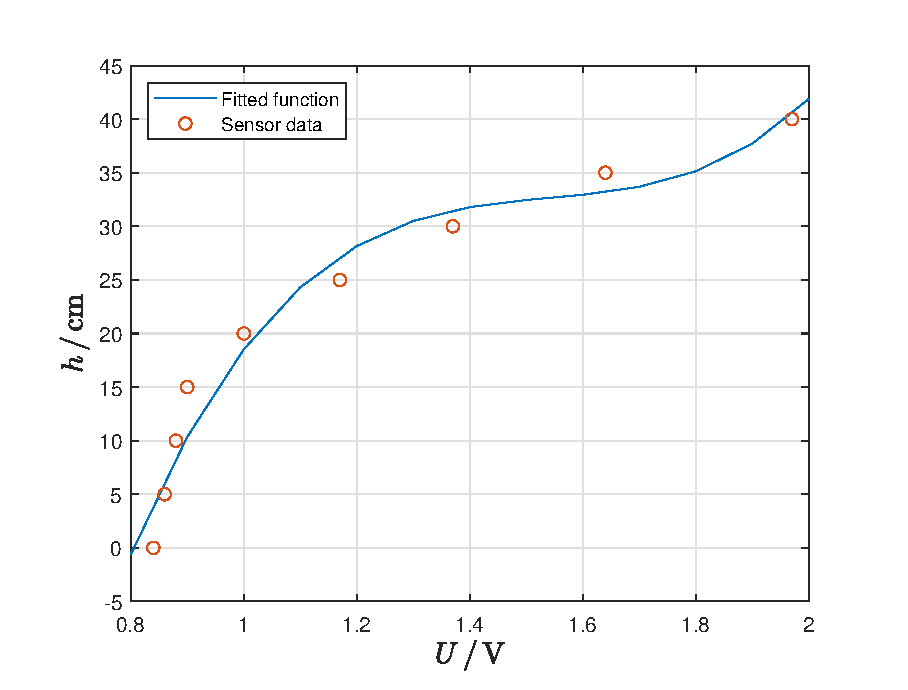
\includegraphics[angle=0,width=0.6\textwidth]{figure/fittedFunction.eps}
    \end{center}
    \caption[Fitted function for first lab preparation]
    {Fitted function $h(u) = (73.36 \cdot u^3) + (-339.13 \cdot u^2) + (527.23 \cdot u) + (-242.94)$}
    \label{fig:fittedFunction}
\end{figure}
\FloatBarrier

\subsection{Second preparation} \label{appendix:secondpreparation}
\FloatBarrier
\begin{figure}[ht]
	\begin{center}
        % trim = left bottom right top
		\includegraphics[clip, trim=0cm 5cm 0cm 5cm, width=1\textwidth]{simulink/simulinkSimulation.pdf}
		\caption[Simulink simulation of the control system]{Simulink simulation of the control system}
		\label{fig:simuSimulation}
	\end{center}
\end{figure}
\FloatBarrier

\FloatBarrier
\begin{figure}[ht]
	\begin{center}
        % trim = left bottom right top
		\includegraphics[clip, trim=0cm 10cm 0cm 8cm, width=1\textwidth]{simulink/simulinkModel.pdf}
		\caption[Simulink model of the system]{Simulink model of the system}
		\label{fig:simuModel}
	\end{center}
\end{figure}
\FloatBarrier

\FloatBarrier
\begin{figure}[ht]
	\begin{center}
        % trim = left bottom right top
		\includegraphics[clip, trim=0cm 8cm 0cm 8cm, width=1\textwidth]{simulink/simulinkController.pdf}
		\caption[Simulink controller]{Simulink controller}
		\label{fig:simuController}
	\end{center}
\end{figure}
\FloatBarrier

\FloatBarrier
\begin{figure}[ht]
	\begin{center}
        % trim = left bottom right top
		\includegraphics[clip, trim=0cm 6.5cm 0cm 6cm, width=1\textwidth]{simulink/simulinkObserver.pdf}
		\caption[Simulink observer]{Simulink observer}
		\label{fig:simuObserver}
	\end{center}
\end{figure}
\FloatBarrier

\FloatBarrier
\begin{figure}[ht]
    \centering
    \begin{subfigure}[b]{0.45\textwidth}
    \includegraphics[width=\textwidth]{simulink/simulinkPlotStepController.eps}
    \caption{}
    \label{subfig:stepController}
    \end{subfigure}
    \begin{subfigure}[b]{0.45\textwidth}
    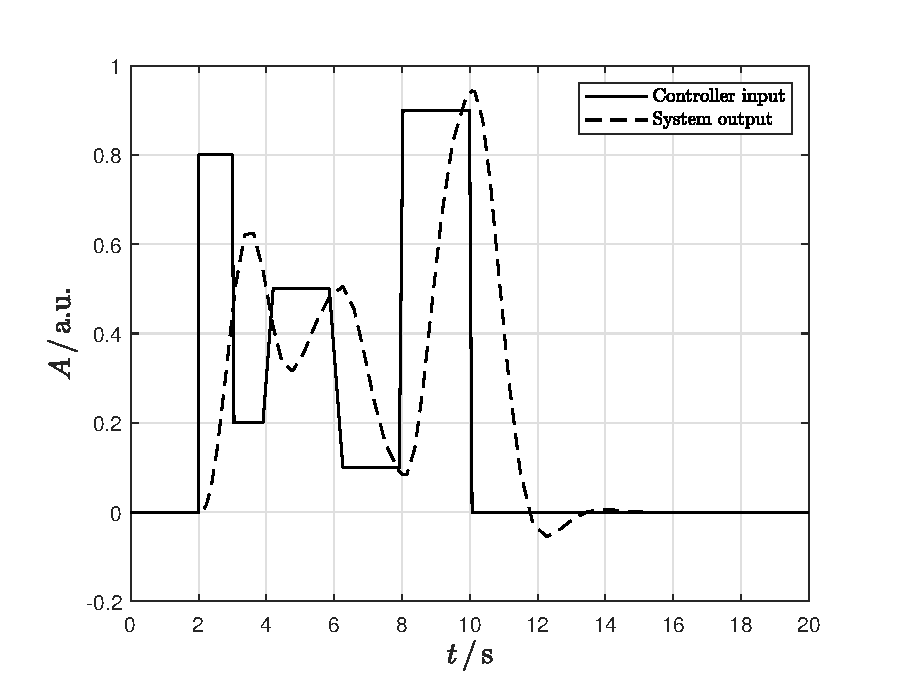
\includegraphics[width=\textwidth]{simulink/simulinkPlotTrajectoryController.eps}
    \caption{}
    \label{subfig:trajController}
    \end{subfigure}

    \hfill
    
    \begin{subfigure}[b]{0.45\textwidth}
    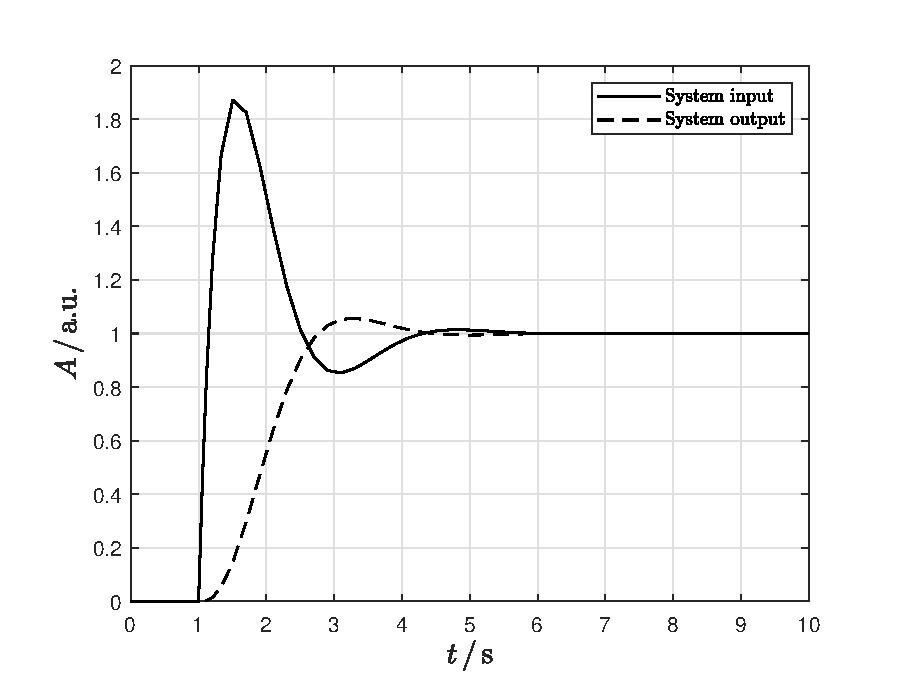
\includegraphics[width=\textwidth]{simulink/simulinkPlotStepSystem.eps}
    \caption{}
    \label{subfig:stepSystem}
    \end{subfigure}
    \begin{subfigure}[b]{0.45\textwidth}
    \includegraphics[width=\textwidth]{simulink/simulinkPlotTrajectorySystem.eps}
    \caption{}
    \label{subfig:trajSystem}
    \end{subfigure}

    \hfill
    
    \begin{subfigure}[b]{0.45\textwidth}
    \includegraphics[width=\textwidth]{simulink/simulinkPlotStepObserver.eps}
    \caption{}
    \label{subfig:stepObserver}
    \end{subfigure}
    \begin{subfigure}[b]{0.45\textwidth}
    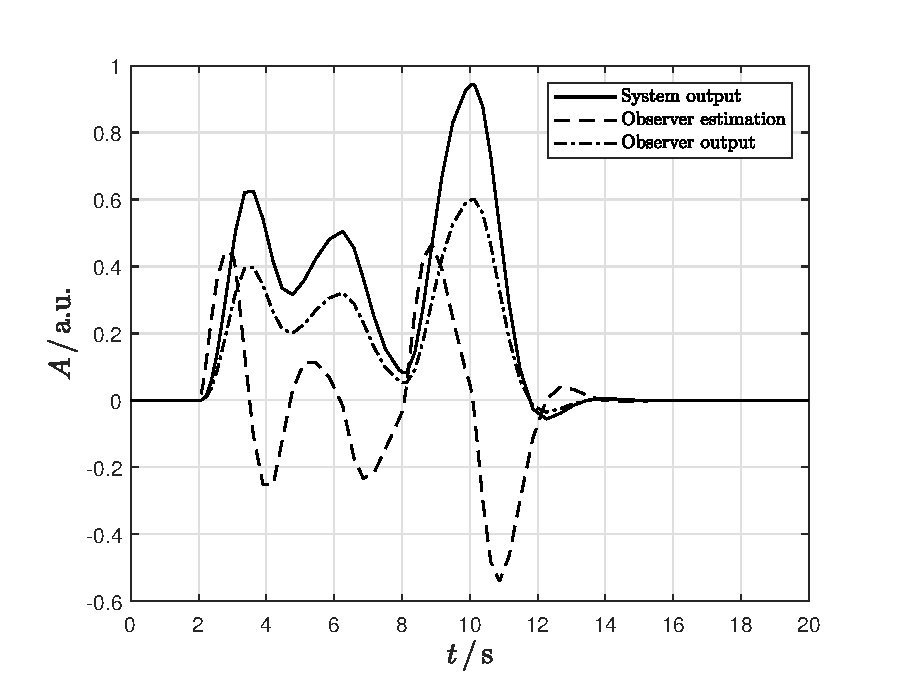
\includegraphics[width=\textwidth]{simulink/simulinkPlotTrajectoryObserver.eps}
    \caption{}
    \label{subfig:trajObserver}
    \end{subfigure}

    \hfill
    
    \caption[Simulations in Simulink]{Left for step input with (a) controller (c) system and (e) observer. Right trajectory input with (b) controller (d) system and (f) observer.}
    \label{fig:simulations}
\end{figure}
\FloatBarrier


\newpage


%========================DATA===================================
\section{Laboratory} \label{appendix:data}

\subsection{Sensor data} \label{appendix:sensordata}
\begin{table}[H]
\caption[Sensor output voltage against distance]{Sensor output voltage against distance} \label{tab:sensor}
\begin{center}
\begin{tabular}{ c c }
\toprule
Distance & Sensor voltage \\
\midrule\\
18  & 1.93 \\
23  & 1.91 \\
28  & 1.68 \\
33  & 1.32 \\
38  & 1.11 \\
43  & 0.96 \\
48  & 0.90 \\
53  & 0.88 \\
58  & 0.82 \\
\bottomrule
\end{tabular} 
\end{center}
\end{table} 

\FloatBarrier
\begin{figure}[ht]
    \begin{center}
    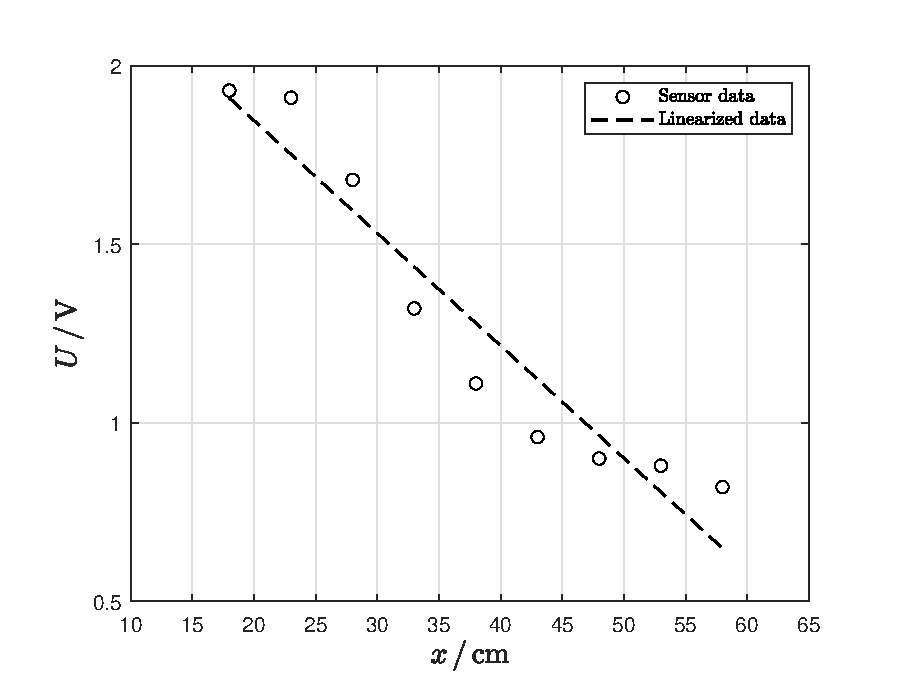
\includegraphics[angle=0,width=0.6\textwidth]{figure/sensorLinearized.eps}
    \end{center}
    \caption[Sensor linearization]
    {Sensor linearization: $f(x) = -0.0315*x + 2.4758888$}
    \label{fig:sensorLinearization}
\end{figure}
\FloatBarrier

\newpage

\subsection{System identification} \label{appendix:systemidentification}
\FloatBarrier
\begin{figure}[ht]
    \centering
    \begin{subfigure}[b]{0.45\textwidth}
    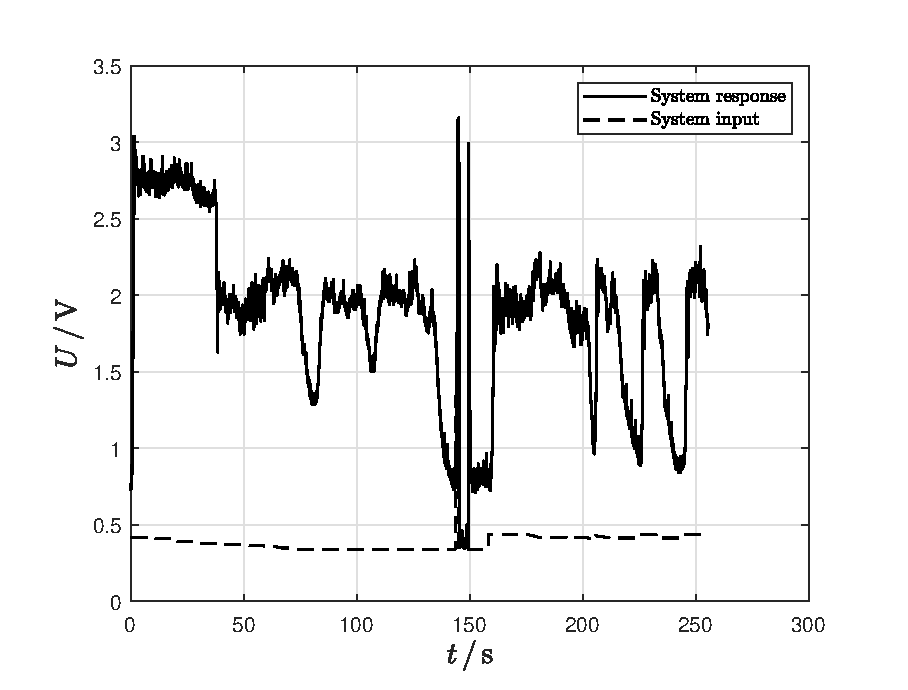
\includegraphics[width=\textwidth]{figure/raw.eps}
    \caption{}
    \label{subfig:raw}
    \end{subfigure}
    \begin{subfigure}[b]{0.45\textwidth}
    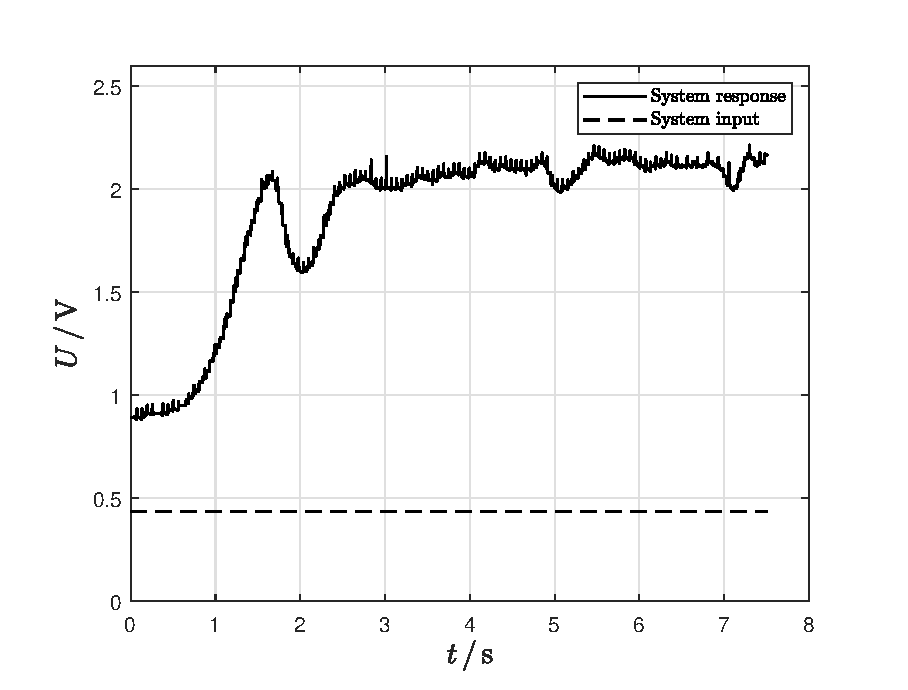
\includegraphics[width=\textwidth]{figure/trimming.eps}
    \caption{}
    \label{subfig:trimming}
    \end{subfigure}

    \hfill
    
    \begin{subfigure}[b]{0.45\textwidth}
    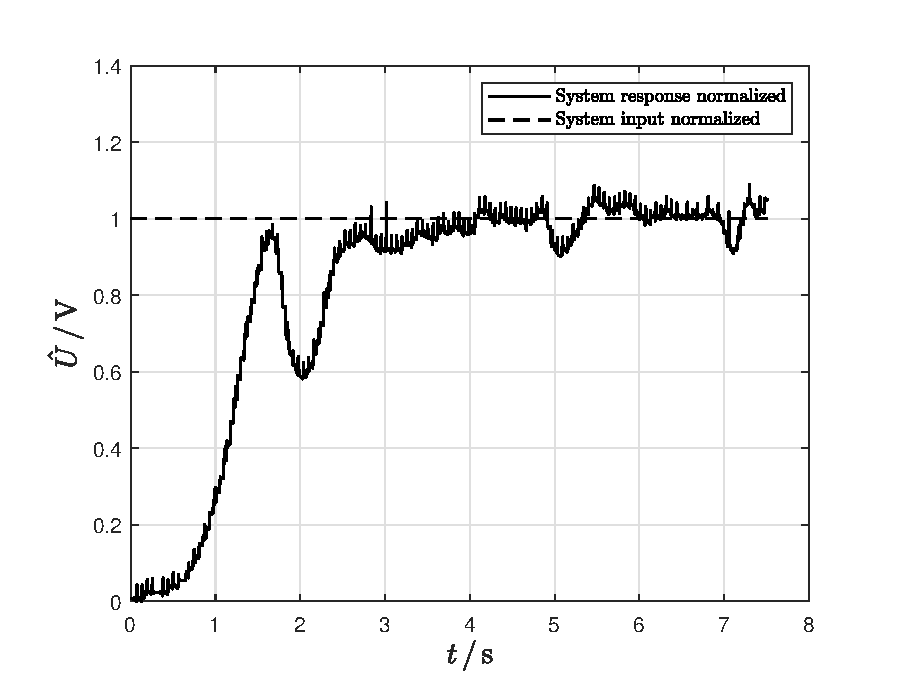
\includegraphics[width=\textwidth]{figure/normalize.eps}
    \caption{}
    \label{subfig:normalize}
    \end{subfigure}
    \begin{subfigure}[b]{0.45\textwidth}
    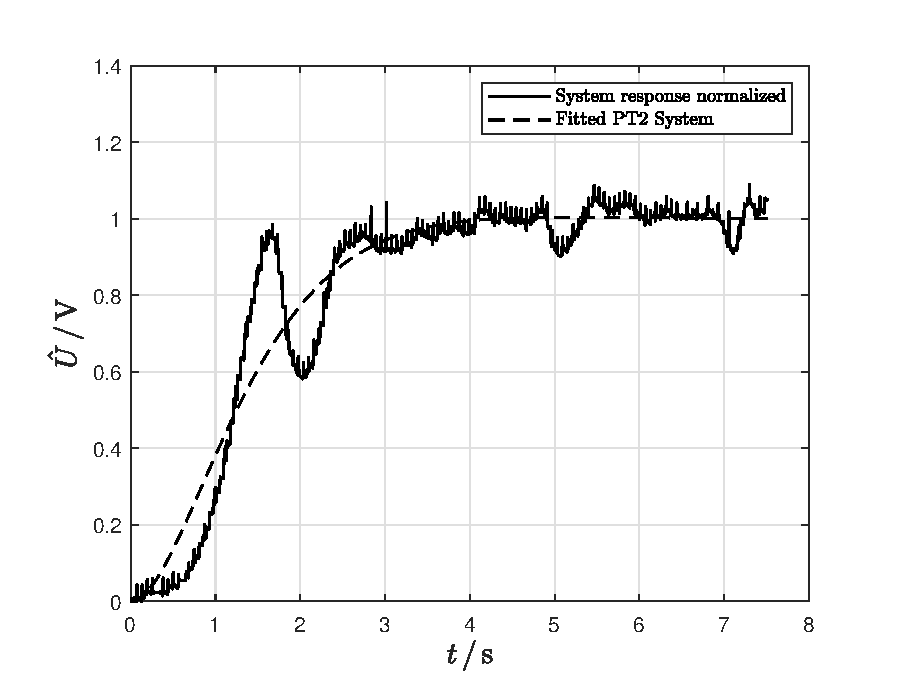
\includegraphics[width=\textwidth]{figure/fitting.eps}
    \caption{}
    \label{subfig:fitting}
    \end{subfigure}

    \hfill
    
    \caption[System identification in the laboratory]{(a) Raw data (b) Trimmed (c) Normalized (d) Fitted PT2 system}
\end{figure}
\FloatBarrier

\newpage

\subsection{Controller performance} \label{appendix:performance}
\FloatBarrier
\begin{figure}[ht]
	\begin{center}
        % trim = left bottom right top
		\includegraphics[clip, trim=0cm 6cm 0cm 6cm, width=0.8\textwidth]{simulink/simulinkLaboratory.pdf}
		\caption[Simulink laboratory application]{Simulink laboratory application}
		\label{fig:simuLaboratory}
	\end{center}
\end{figure}
\FloatBarrier

\FloatBarrier
\begin{figure}[ht]
    \begin{center}
    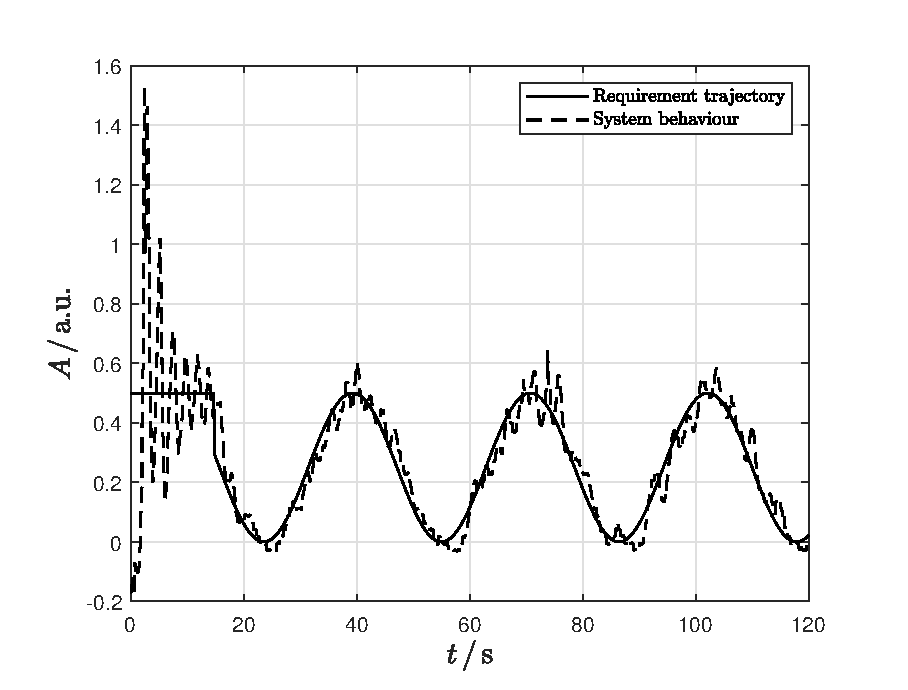
\includegraphics[angle=0,width=0.6\textwidth]{simulink/simulinkPlotTrajectoryLaboratory.eps}
    \end{center}
    \caption[System behaviour with sine wave trajectory]
    {System behaviour with sine wave trajectory}
    \label{fig:simuSineTrajectory}
\end{figure}
\FloatBarrier


\newpage


%========================MATLAB===================================
\section{MATLAB} \label{appendix:matlab}

\subsection{First laboratory}
\lstinputlisting[style=MStyle]{m_files/laboratory.m}
\subsubsection{Plots}
\lstinputlisting[style=MStyle]{m_files/plots.m}
\subsubsection{PT2 fitting function}
\lstinputlisting[style=MStyle]{m_files/unit_step_PT2.m}

\newpage

\subsection{Second laboratory}
\lstinputlisting[style=MStyle]{m_files/laboratory1.m} 

% letzte Fußzeile (MCI Logo)
\pagestyle{fancy}
\lfoot{\includegraphics[height=0.9cm]{Images/MCIFuss.png}}
\newpage
\lfoot{}

\end{document}